\section{Machine Learning Workloads} \label{sec-ml-workloads}
We define a machine learning workload as a series of exploratory data analysis steps followed by one or multiple model building steps.
Typically users analyze the data by first performing different transformations to gain insight into the data.
Then, based on these analyses, they apply the right set of transformations to the data to train one or multiple models on the transformed training data.
Therefore, machine learning workloads typically consist of both interactive (exploratory analysis) and long-running processes (hyperparameter tuning and model training).
Using the experiment database, we can speed up the execution of the machine learning workloads.
By analyzing the experiment database, we can extract the common transformations on data and materialize them.
Thus, during the interactive exploratory analysis, we first analyze the workload to look for reuse opportunities and return the materialized data when possible.
Moreover, using the experiment database, we provide the users with already trained models or promising hyperparameters which decreases the execution time of the hyperparameter search and model training.

We analyzed several scripts from the Titanic: Machine Learning from Disaster competition in Kaggle\footnote{https://www.kaggle.com/c/titanic}.
The Kaggle platform allows users to submit their solutions as scripts (called notebooks or kernels) to the Kaggle platform.
These notebooks are available publicly for other users to view and fork in their own workspace.
Figure \ref{fig-titanic-script-hierarchy} shows some of the popular notebooks and how other users wrote their notebooks based on the existing ones.
The numbers show how many times each script is forked.
The top most-voted notebooks for the Titanic competition have been forked a total of 44,434 times.
This demonstrates that many of the workloads share similar sets of data transformations and model training.
Materializing frequent transformations and models can greatly increase the efficiency and many repeated operations can be avoided.

\begin{figure}
\centering
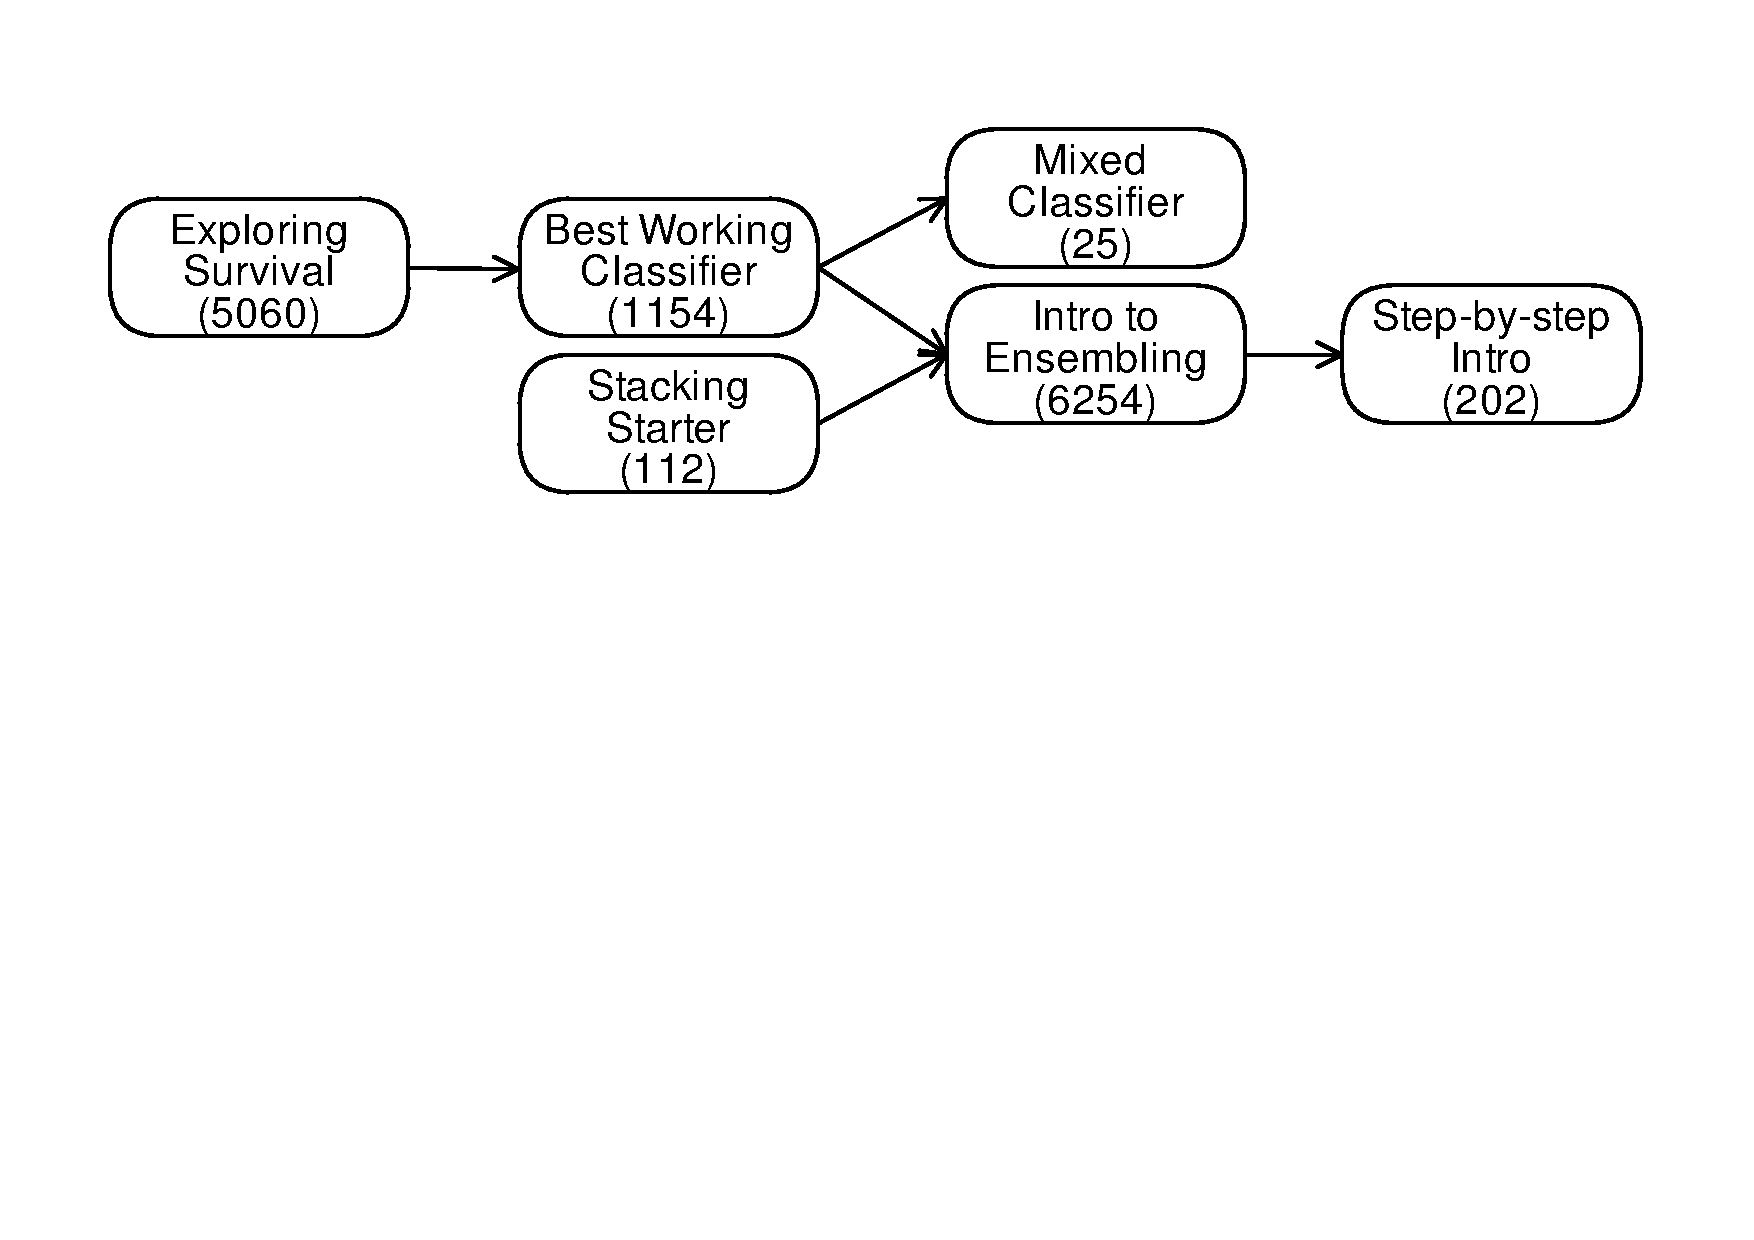
\includegraphics[width=\columnwidth]{../images/kaggle-titanic-scripts-graph}
\caption{The fork hierarchy of some of the popular notebooks in Kaggle's Titanic competition and how many times each notebook is forked}
\label{fig-titanic-script-hierarchy}
\end{figure}

In order to apply the materialization optimization, we first define the characteristics of the machine learning workloads.
Then, we specify how to detect reuse opportunities from the experiment database.

\subsection{Machine Learning Workload Characteristics}
We assume the main units of work are dataframe like objects that contain one or many columns, where all the data items in one column are of one data type.
We divide the operations in the ML workloads into 2 categories.

\begin{table}
\centering
\begin{tabular}{ll}
\hline
	   Feature Extraction & Feature Selection\\ \hline
        feature hasher & variance threshold  \\
        one hot encoding & select k best \\
        count vectorizer& select percentile \\ 
        tfidf transformer & recursive feature elimination \\
        hashing vectorizer & select from model \\
        extract\_patch\_2d &  \\
        \hline
\end{tabular}
\caption{List of feature extraction and feature selection operations}\label{feature-engineering-operations}
\end{table}

\textbf{1. Feature engineering:}
\begin{itemize}
\item feature selection operations
\item feature extraction operations
\item user-defined feature engineering operations
\end{itemize}

Table \ref{feature-engineering-operations} shows the list common feature extraction and feature selection operations.

\textbf{2. Model building: }
\begin{itemize}
\item model training operation that applies a training algorithm to a dataset
\item common aggregation operations (such as mean, max, min, and percentile)
\item user-defined aggregation operations 
\end{itemize}
Each model building operation results in objects that can either be used in other feature engineering operations (applying PCA to data or categorizing a column based on values in percentile aggregate) or can be a complete machine learning model that can be used to make predictions on unseen data.
\todo[inline]{How can we capture these in the graph? maybe special edges that connect these nodes to a data node? }

%%% Continue from here
\subsection{Graph Representation}\label{sub-graph-construction}
In order to efficiently apply our proposed optimizations, we utilize a graph model to store the meta-data and logs of machine learning workloads.
We let $\mathcal{V}=\{v_i\}, i = 1, \cdots, n$ to be a collection of artifacts that exist in the experiment database, where each artifact is either a raw dataset, a pre-processed dataset resulting from a feature engineering operation, or a model resulting from a model building operation.
We let $\mathcal{E}=\{e_i\}, i = 1, \cdots, n$ to be a collection of executed operations that exist in the experiment database.
A directed edge $e$ from $v_i$ to $v_j$ in $\mathcal{G}(\mathcal{V},\mathcal{E})$ indicates that the artifact $v_j$ is the result of applying the operation $e$ to the artifact $v_i$.
Every vertex is labeled by $<s>$, which represents the storage size of artifact when materialized.
Every edge is labeled by $\langle f, t\rangle$, where $f$ represents the frequency of the operation (the number of times the operation has been executed) and $t$ represent the average run time (in seconds) of the operation.
Similarly, when a machine learning workload is executed, we extended the graph to capture the new feature engineering and model building operations.
If an operation already exists in the graph, we update the frequency and average run time attributes.
Otherwise, we add a new edge and vertex, representing the new operation and the generated artifact, to the experiment graph.


%The process of constructing the graph is as follows.
%First, a (root) node which represents the (training) dataset is created.
%Since operations are performed on columns of the dataset, an edge is drawn for every column of the data from the root to new vertices representing every column of the dataset.
%Every operation represents an edge.
%An edge connects a starting node (one or more columns of the data) to another node (the resulting columns).
%If the feature engineering operation is not user-defined, the edge also stores information about the feature engineering operation applied.
%The resulting node of the operation contains the columns of data resulted from applying the operation.
%
%Model building operations also operate on one or more columns of the data.
%Similar to the feature engineering operation, an edge represents the operation.
%If the operation is not an user-defined aggregation operation, the edge carries information about the operation (such as training algorithm and hyper-parameters).
%The resulting node represents a machine learning model (for model training operations) or data structures for keeping the aggregated values (for aggregation operations).

Figure \ref{fig-experiment-graph} shows an example graph constructed from the code in Listing \ref{listing-experiment-graph} based on the Avito demand prediction challenge \footnote{https://www.kaggle.com/c/avito-demand-prediction/}.

\begin{lstlisting}[language=Python, caption=Example script,captionpos=b,label = {listing-experiment-graph}]
import numpy as np
import pandas as pd

from sklearn import svm
from sklearn.feature_selection import SelectKBest
from sklearn.feature_extraction.text import CountVectorizer

train = pd.read_csv('../input/train.csv') 
print train.columns # [ad_desc,ts,u_id,price,y]
vectorizer = CountVectorizer()
count_vectorized = vectorizer.fit_transform(train['ad_desc'])
selector =  SelectKBest(k=2)
top_features = selector.fit_transform(train[['ts','u_id','price']], 
				      train['y'])
X = pd.concat([count_vectorized,top_features], axis = 1)
model = svm.SVC()
model.fit(X, train['y'])
\end{lstlisting}

\begin{figure}
\centering
\documentclass{standalone}
\usepackage{tikz}
\usetikzlibrary{graphdrawing, graphs, quotes, positioning,arrows, backgrounds, math, calc, shapes, positioning}
\usegdlibrary{trees}
\begin{document}
\begin{tikzpicture}
%\draw[help lines]  (-2,0) grid (6,6);
\tikzstyle{every node}=[inner sep=0.02cm]
\node (train) [ellipse, draw] at (3,6) {\normalsize $train$};
% layer 1
\node (ad) [ellipse, draw]  at (0,5.5){\normalsize $ad\_desc$};
\node (forselection) [ellipse, draw] at (3.5,5.4) {\normalsize $t\_subset$};
\node (y) [ellipse, draw] at (5.5, 5.5){\normalsize $y$};
% layer 2
\node (cv) [ellipse, draw] at (1,4.9) {\normalsize $cnt\_vect$};
\node(sk) [ellipse, draw]  at (4,4.6){\normalsize $top\_feats$};
% layer 3
%\node (merged1) [circle, draw] at (1.5, 3.5) {$v_6$};
\node (cvsk) [ellipse, draw] at (3.7,3.8) {\normalsize$X$};
% layer 4
%\node(merged2) [circle, draw] at (3, 2.8) {$v_8$};
% layer 5
\node(model) [ellipse, draw, fill=green!20] at (4.9, 3.5)  {$model$};

\graph [grow down,edge quotes ={inner sep=1pt}, edges ={thick},radius=.2cm, nodes={circle, draw,font =\small}]{
(train) [label=train]
->  (ad)
-> (cv)
%-> [anchor=east,align=center,"m"](merged1) 
->(cvsk) 
%-> [anchor=south, align=center,"m"](merged2) ;
-> (model);

(train) 
-> (forselection)
-> (sk)
-> (cvsk) ;

(train) 
->    (y)
%-> [anchor=west, align=center,"m"](merged2) 
->  (model);
};
\end{tikzpicture}
\end{document}
\caption{Experiment graph constructed from the Listing \ref{listing-experiment-graph}}
\label{fig-experiment-graph}
\end{figure}

We make two important assumptions when constructing the graph from the workloads.
First, most of the operations are applied to one or a subset of the columns of a dataset.
In this case, we augment the graph with an edge representing a projection operation that selects the required subset of the columns.
The run-time ($t$) attribute of this edge is set to 0 as this operation is never actually executed.
Second, multiple edges merging into one vertex indicates an operation the receives as input multiple artifacts and outputs one artifact.
This is a critical assumption for our materialization algorithm in Section \ref{sec-materializaiton-and-reuse}.
Currently, we support three types of merge operations:
\begin{itemize}
\item \textbf{concat}: a physical operation that concatenates the columns of the input datasets (e.g., concatenation of $v_4$ and $v_5$ in Figure \ref{fig-experiment-graph} which represents Pandas' \textit{concat} operation).
\item \textbf{join}: a physical operation that joins multiple datasets on a given key.
\item \textbf{combine}: a logical operation that combines the input datasets. The combine operation is used to simplify the representation of operations that require multiple artifacts as input (e.g., combining $v_6$ and $v_3$ in Figure \ref{fig-experiment-graph} which simplifies the representation of \textit{model.fit} of sklearn library).
\end{itemize}
Since the \textit{combine} operation is logical, the run-time attribute ($t$) of every participating edge is set to $0$.
For \textit{join} and \textit{concat} operations, for every participating edge, the frequency is set to the total number of times the merge operation executed.
While, the run-time of every participating edge is set to the total run-time divided by the number of the participating edges (e.g., in Figure \ref{fig-experiment-graph}, if the \textit{concat} operation between $v_4$ and $v_5$ is executed 6 times with an average run-time of 10 seconds, the edges connecting $v_4$ to $v_6$ and $v_5$ to $v_6$ have the label $\langle6, 5\rangle$).

It is important to note that a given workload does not necessarily need to include a complete set of transformations, machine learning models, and hyperparameters.
This indicates that a simple dataset load is also considered a workload, upon the execution of which a node is added to the experiment graph.